%% This is file `elsarticle-template-1-num.tex',
%%
%% Copyright 2009 Elsevier Ltd
%%
%% This file is part of the 'Elsarticle Bundle'.
%% ---------------------------------------------
%%
%% It may be distributed under the conditions of the LaTeX Project Public
%% License, either version 1.2 of this license or (at your option) any
%% later version.  The latest version of this license is in
%%    http://www.latex-project.org/lppl.txt
%% and version 1.2 or later is part of all distributions of LaTeX
%% version 1999/12/01 or later.
%%
%% The list of all files belonging to the 'Elsarticle Bundle' is
%% given in the file `manifest.txt'.
%%
%% Template article for Elsevier's document class `elsarticle'
%% with numbered style bibliographic references
%%
%% $Id: elsarticle-template-1-num.tex 149 2009-10-08 05:01:15Z rishi $
%% $URL: http://lenova.river-valley.com/svn/elsbst/trunk/elsarticle-template-1-num.tex $
%%
\documentclass[preprint,12pt]{elsarticle}

%% Use the option review to obtain double line spacing
%% \documentclass[preprint,review,12pt]{elsarticle}

%% Use the options 1p,twocolumn; 3p; 3p,twocolumn; 5p; or 5p,twocolumn
%% for a journal layout:
%% \documentclass[final,1p,times]{elsarticle}
%% \documentclass[final,1p,times,twocolumn]{elsarticle}
%% \documentclass[final,3p,times]{elsarticle}
%% \documentclass[final,3p,times,twocolumn]{elsarticle}
%% \documentclass[final,5p,times]{elsarticle}
%% \documentclass[final,5p,times,twocolumn]{elsarticle}

%% if you use PostScript figures in your article
%% use the graphics package for simple commands
%% \usepackage{graphics}
%% or use the graphicx package for more complicated commands
%% \usepackage{graphicx}
%% or use the epsfig package if you prefer to use the old commands
%% \usepackage{epsfig}

%% The amssymb package provides various useful mathematical symbols
\usepackage{amssymb}
%% The amsthm package provides extended theorem environments
%% \usepackage{amsthm}

%% The lineno packages adds line numbers. Start line numbering with
%% \begin{linenumbers}, end it with \end{linenumbers}. Or switch it on
%% for the whole article with \linenumbers after \end{frontmatter}.
\usepackage{lineno}
\usepackage{hyperref}

%% natbib.sty is loaded by default. However, natbib options can be
%% provided with \biboptions{...} command. Following options are
%% valid:

%%   round  -  round parentheses are used (default)
%%   square -  square brackets are used   [option]
%%   curly  -  curly braces are used      {option}
%%   angle  -  angle brackets are used    <option>
%%   semicolon  -  multiple citations separated by semi-colon
%%   colon  - same as semicolon, an earlier confusion
%%   comma  -  separated by comma
%%   numbers-  selects numerical citations
%%   super  -  numerical citations as superscripts
%%   sort   -  sorts multiple citations according to order in ref. list
%%   sort&compress   -  like sort, but also compresses numerical citations
%%   compress - compresses without sorting
%%
%% \biboptions{comma,round}

% \biboptions{}


\journal{GSoC KDE 2017}

\begin{document}

\begin{frontmatter}

%% Title, authors and addresses

%% use the tnoteref command within \title for footnotes;
%% use the tnotetext command for the associated footnote;
%% use the fnref command within \author or \address for footnotes;
%% use the fntext command for the associated footnote;
%% use the corref command within \author for corresponding author footnotes;
%% use the cortext command for the associated footnote;
%% use the ead command for the email address,
%% and the form \ead[url] for the home page:
%%
%% \title{Title\tnoteref{label1}}
%% \tnotetext[label1]{}
%% \author{Name\corref{cor1}\fnref{label2}}
%% \ead{email address}
%% \ead[url]{home page}
%% \fntext[label2]{}
%% \cortext[cor1]{}
%% \address{Address\fnref{label3}}
%% \fntext[label3]{}

\title{Porting activities in GCompris in Qt-Quick}

%% use optional labels to link authors explicitly to addresses:
%% \author[label1,label2]{<author name>}
%% \address[label1]{<address>}
%% \address[label2]{<address>}

\author{Rudra Nil Basu}

\address{ \textbf{Email ID}: rudra.nil.basu.1996@gmail.com}
\address{ \textbf{Freenode IRC Nick}: rudra}
\address{ \textbf{Location}: Kolkata, West Bengal, India UTC+5.30}
\address{ \textbf{Mentor}: Bruno Coudoin (bruno.coudoin@gcompris.net)}
\address{ \textbf{Co-Mentor}: Johnny Jazeix (jazeix@gmail.com), }

\end{frontmatter}

%%
%% Start line numbering here if you want
%%
%\linenumbers

%% main text
\section{Motivation}
\label{S:1}

GCompris is about teaching the basics in the most easiest way to children between the age of 2 to 10. The gtk+ version of GCompris was very well recieved, and from there it was decided to Qt version, to make GCompris available for all kinds of devices, like tablets. The latest version of GCompris is 0.70 and as of now it has 137 categories on various topics like science, maths, games and much more, fully supporting 15 languages.




%As of \today , a brief statistics of GCompris are:
%\begin{itemize}
%\item Latest Version: 0.70
%\item A total of 137 categories on various topics like science, maths, games and much more.
%\item 15 languages fully supported
%\item More than 100000 downloads on the Google Play Store
%\item The new version contains 8 new activities
%\end{itemize}

My goal for the project is to port two experimental activities from the Gtk+ version of GCompris to the Qt version.

The best way to teach any concept is by demonstration. But it is not always possible to demonstrate everything that needs to be taught, such as the working of submarine and it's different parts. That's were simulation of real world problems come to play. The aim of this project is to simulate real world situations in two activities, \textit{"Pilot a Submarine"} and \textit{"Sea race (Single Player)"}

\section{Project Goals}
\label{S:1}

By the end of the Google Summer of Code's time period, I will be completing the following activities :

\begin{itemize}

\item \textbf{Pilot a Submarine}: It is a port to the Qt version of a strategic activity originally present in the Gtk+ version aimed to teach how a submarine works. It was started in this branch: 

\href{https://cgit.kde.org/gcompris.git/log/?h=gsoc-submarine}{https://cgit.kde.org/gcompris.git/log/?h=gsoc-submarine}

\item \textbf{Sea Race (2 players)}: It is an experimental activity from the Gtk+ version, which will be ported to the Qt version of GCompris. This activity is aimed at learning how to enter commands into a computer, providing an introduction to the concepts of programming to children. It was originally present in the Gtk+ version:

\href{https://github.com/gcompris/GCompris-gtk/tree/master/src/searace-activity}{https://github.com/gcompris/GCompris-gtk/tree/master/src/searace-activity}

\item \textbf{The Solar System}: This activity aims at providing a basic understanding about our Solar System, it's planets and facts and properties of each of the planets.
\end{itemize}

\section{Implementation Details}
\label{S:1}

\subsection{Pilot a Submarine}

The  \textit{"Pilot a Submarine"} is to learn how a submarine works, explaining the usage of elements such as engine, rudders and air tanks, in order to navigate a submarine to a required depth.

\begin{itemize}


\item Since this activity was already present in the Gtk+ version, I will be using the svg and the audio files from the resources used in the Gtk+ submarines activity. This will allow me to dive into the coding part directly. 

\item There will be a tutorial at the start of the activity, which will give a brief description about the different elements (engine, rudders and air tanks) and it's functions.

\item Firstly I will be implementing the submarine and the mechanics of it's elements, namely the engine, rudders and the air tanks. Once that is in place, I will then shift on to create various levels and it's variations.

%The Gtk+ version had only 4 levels, and I will increase the number of levels in the Qt port, increasing the difficulty curve, bringing up elements like caves, rocks, while still keeping it doable for children within the prescribed age limit.

\item The activity will contain pickups in the form of jewels, as it was present in the Gtk+ version

\item Besides the regular pickups in the Gtk+ version, there will be additional threats in the form of rocks and caves, in order to maintain an increasing difficulty curve, while still keeping it doable for children within the prescribed age limit.

\item In order to enhance the experience, the overall activity and the movement of the submarine and the animations will be smoother compared to the Gtk+ activity.

\begin{figure}[h]
\centering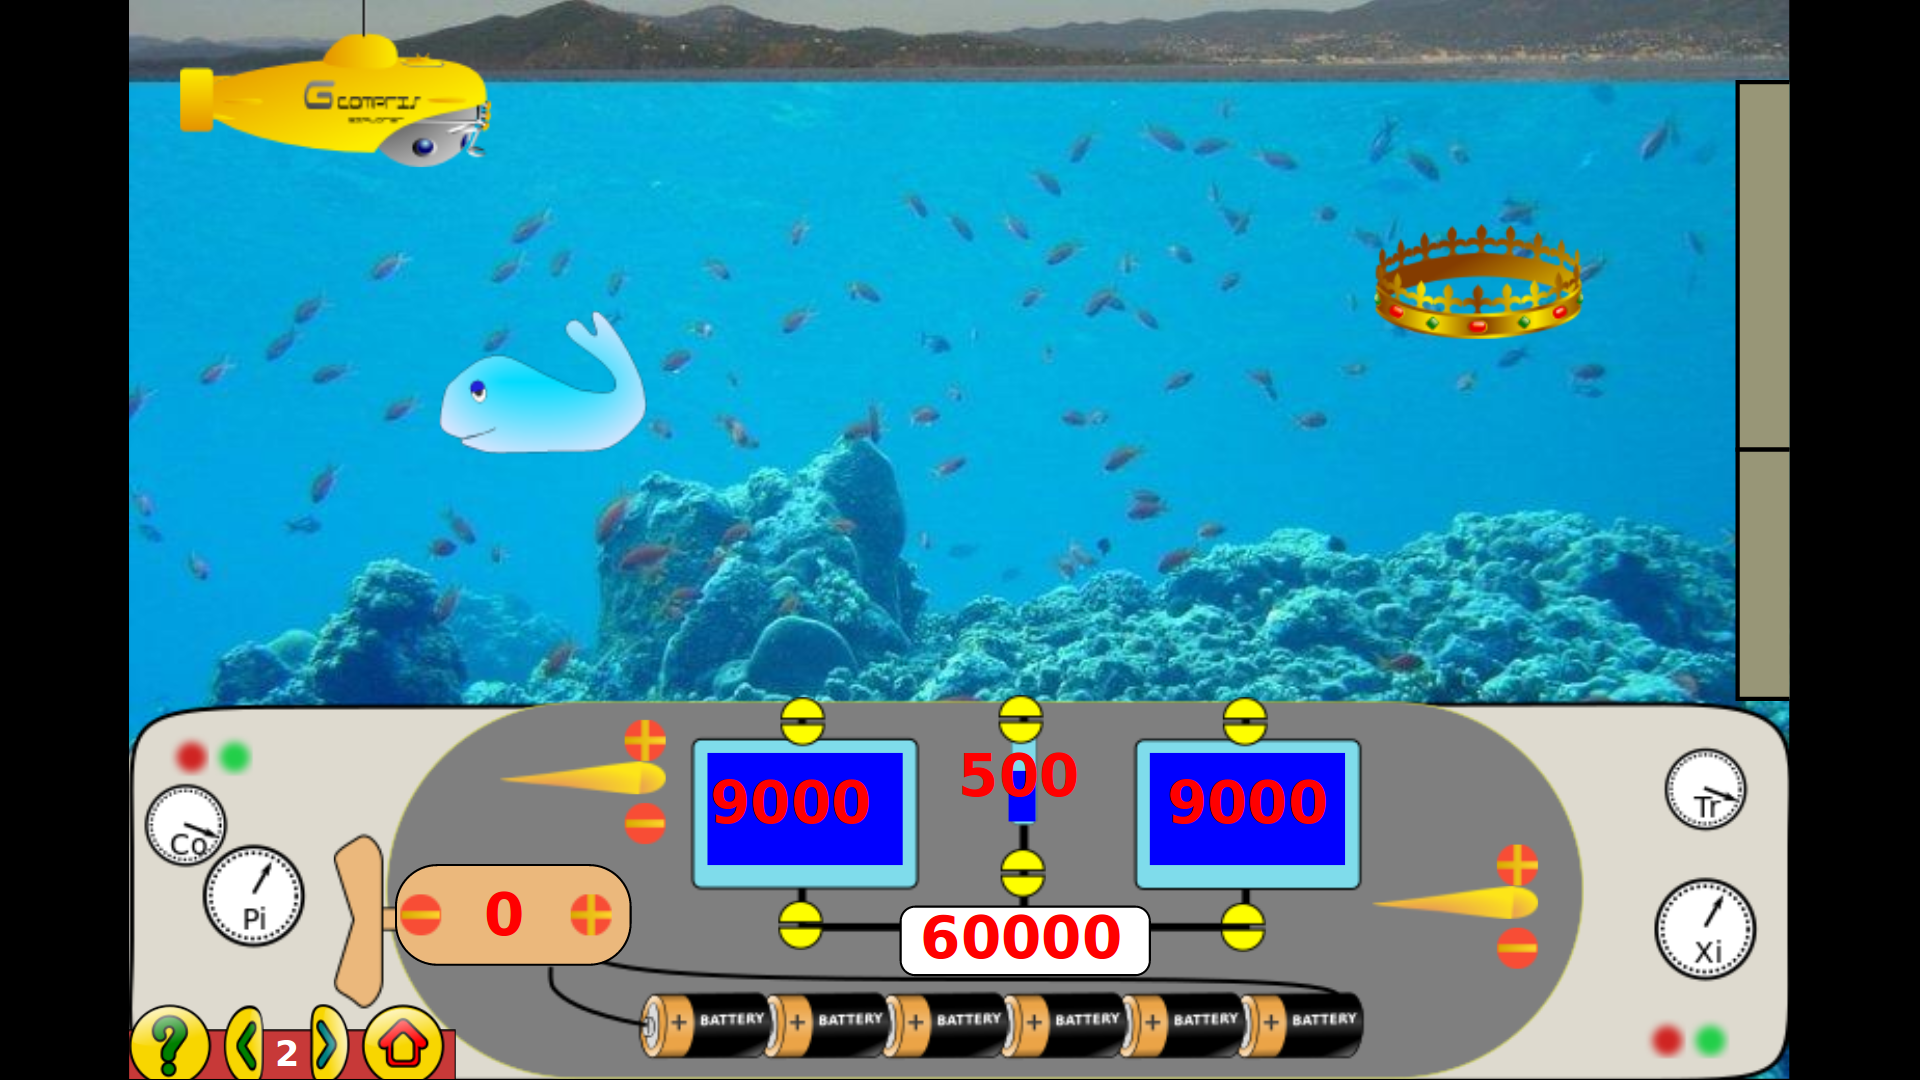
\includegraphics[width=1.0\linewidth]{submarine}
\caption{Submarine Activity}
\end{figure}

\end{itemize}
\subsection{Sea Race (Single Player)}


\subsection{Third undecided one}
/*2d matrix, Tux, door and few pickups. command tux to take all pickups and move out of the door. Commands - rotate (+-90, +180), move forward (x blocks)*/

/*Physics*/

/*Complete incomplete activities*/

\section{Timeline}
\label{S:1}

\section{About Me}
\label{S:1}

\begin{enumerate}
\item Numbered list item one
\item Numbered list item two
\end{enumerate}

\subsection{Subsection One}

Quisque elit ipsum, porttitor et imperdiet in, facilisis ac diam. Nunc facilisis interdum felis eget tincidunt. In condimentum fermentum leo, non consequat leo imperdiet pharetra. Fusce ac massa ipsum, vel convallis diam. Quisque eget turpis felis. Curabitur posuere, risus eu placerat porttitor, magna metus mollis ipsum, eu volutpat nisl erat ac justo. Nullam semper, mi at iaculis viverra, nunc velit iaculis nunc, eu tempor ligula eros in nulla. Aenean dapibus eleifend convallis. Cras ut libero tellus. Integer mollis eros eget risus malesuada fringilla mattis leo facilisis. Etiam interdum turpis eget odio ultricies sed convallis magna accumsan. Morbi in leo a mauris sollicitudin molestie at non nisl.

\begin{table}[h]
\centering
\begin{tabular}{l l l}
\hline
\textbf{Treatments} & \textbf{Response 1} & \textbf{Response 2}\\
\hline
Treatment 1 & 0.0003262 & 0.562 \\
Treatment 2 & 0.0015681 & 0.910 \\
Treatment 3 & 0.0009271 & 0.296 \\
\hline
\end{tabular}
\caption{Table caption}
\end{table}

\subsection{Subsection Two}

Donec eget ligula venenatis est posuere eleifend in sit amet diam. Vestibulum sollicitudin mauris ac augue blandit ultricies. Nulla facilisi. Etiam ut turpis nunc. Praesent leo orci, tincidunt vitae feugiat eu, feugiat a massa. Duis mauris ipsum, tempor vel condimentum nec, suscipit non mi. Fusce quis urna dictum felis posuere sagittis ac sit amet erat. In in ultrices lectus. Nulla vitae ipsum lectus, a gravida erat. Etiam quam nisl, blandit ut porta in, accumsan a nibh. Phasellus sodales euismod dolor sit amet elementum. Phasellus varius placerat erat, nec gravida libero pellentesque id. Fusce nisi ante, euismod nec cursus at, suscipit a enim. Nulla facilisi.

\begin{figure}[h]
\centering
\includegraphics[width=0.4\linewidth]{placeholder}
\caption{Figure caption}
\end{figure}

Integer risus dui, condimentum et gravida vitae, adipiscing et enim. Aliquam erat volutpat. Pellentesque diam sapien, egestas eget gravida ut, tempor eu nulla. Vestibulum mollis pretium lacus eget venenatis. Fusce gravida nisl quis est molestie eu luctus ipsum pretium. Maecenas non eros lorem, vel adipiscing odio. Etiam dolor risus, mattis in pellentesque id, pellentesque eu nibh. Mauris nec ante at orci ultricies placerat ac non massa. Aenean imperdiet, ante eu sollicitudin vestibulum, dolor felis dapibus arcu, sit amet fermentum urna nibh sit amet mauris. Suspendisse adipiscing mollis dolor quis lobortis.

\begin{equation}
\label{eq:emc}
e = mc^2
\end{equation}

\section{The Second Section}
\label{S:2}

Reference to Section \ref{S:1}. Etiam congue sollicitudin diam non porttitor. Etiam turpis nulla, auctor a pretium non, luctus quis ipsum. Fusce pretium gravida libero non accumsan. Donec eget augue ut nulla placerat hendrerit ac ut mi. Phasellus euismod ornare mollis. Proin tempus fringilla ultricies. Donec pretium feugiat libero quis convallis. Nam interdum ante sed magna congue eu semper tellus sagittis. Curabitur eu augue elit.

Aenean eleifend purus et massa consequat facilisis. Etiam volutpat placerat dignissim. Ut nec nibh nulla. Aliquam erat volutpat. Nam at massa velit, eu malesuada augue. Maecenas sit amet nunc mauris. Maecenas eu ligula quis turpis molestie elementum nec at est. Sed adipiscing neque ac sapien viverra sit amet vestibulum arcu rhoncus.

Vivamus pharetra nibh in orci euismod congue. Pellentesque habitant morbi tristique senectus et netus et malesuada fames ac turpis egestas. Quisque lacus diam, congue vel laoreet id, iaculis eu sapien. In id risus ac leo pellentesque pellentesque et in dui. Etiam tincidunt quam ut ante vestibulum ultricies. Nam at rutrum lectus. Aenean non justo tortor, nec mattis justo. Aliquam erat volutpat. Nullam ac viverra augue. In tempus venenatis nibh quis semper. Maecenas ac nisl eu ligula dictum lobortis. Sed lacus ante, tempor eu dictum eu, accumsan in velit. Integer accumsan convallis porttitor. Maecenas pretium tincidunt metus sit amet gravida. Maecenas pretium blandit felis, ac interdum ante semper sed.

In auctor ultrices elit, vel feugiat ligula aliquam sed. Curabitur aliquam elit sed dui rhoncus consectetur. Cras elit ipsum, lobortis a tempor at, viverra vitae mi. Cras sed urna sed eros bibendum faucibus. Morbi vel leo orci, vel faucibus orci. Vivamus urna nisl, sodales vitae posuere in, tempus vel tellus. Donec magna est, luctus non commodo sit amet, placerat et enim.

%% The Appendices part is started with the command \appendix;
%% appendix sections are then done as normal sections
%% \appendix

%% \section{}
%% \label{}

%% References
%%
%% Following citation commands can be used in the body text:
%% Usage of \cite is as follows:
%%   \cite{key}          ==>>  [#]
%%   \cite[chap. 2]{key} ==>>  [#, chap. 2]
%%   \citet{key}         ==>>  Author [#]

%% References with bibTeX database:

\bibliographystyle{model1-num-names}
\bibliography{sample.bib}

%% Authors are advised to submit their bibtex database files. They are
%% requested to list a bibtex style file in the manuscript if they do
%% not want to use model1-num-names.bst.

%% References without bibTeX database:

% \begin{thebibliography}{00}

%% \bibitem must have the following form:
%%   \bibitem{key}...
%%

% \bibitem{}

% \end{thebibliography}


\end{document}

%%
%% End of file `elsarticle-template-1-num.tex'.
